\section{Evaluation}\marginnote{VTN}
    \subsection{Implementation}\marginnote{VTN}
    All experiments were executed on free tier Google Colab virtual machine which gives 12 GB of RAM. We chose to use TenSEAL and numpy to perform encryption and arithmetic operations on the data. Before encrypting the data, we need to clarify some important parameters which are needed for encryption:
    \begin{itemize}[nosep]
        \item[-] \texttt{coeff\_mod\_bit\_sizes} is a list of numbers. The first number and the last number decide the precision of the decrypted result. Each of the remaining numbers decides the bit size of a result each time we apply multiplication on the encrypted data.
        \item[-] \texttt{poly\_modulus\_degree} is a positive power of 2. The larger the value is, the more complicated encrypted computations it allows; however, the slower the operations are. The value selection of \texttt{poly\_modulus\_degree} depends on the value of \linebreak \texttt{coeff\_mod\_bit\_sizes}. See figure \ref{fig:coeffpolytable}. For example: if \texttt{coeff\_mod\_bit\_sizes} = [40, 20, 40], the total of coefficient mod bit sizes is 100; so that we have to chose the value $4096$ of \texttt{poly\_modulus\_degree} which correspond to the value $109$ of the \texttt{max coeff\_modulus bit-length}.
        \item[-] \texttt{global\_scale} determines the bit-precision of the encoding, so that it affects the precision of the result.
    \end{itemize}
    
    \begin{figure}[ht]
        \centering
        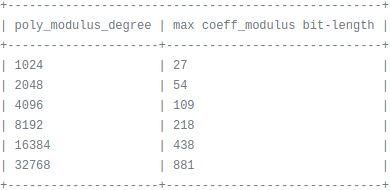
\includegraphics[width=0.5\linewidth]{images/Screenshot from 2021-10-05 23-37-47.png}
        \caption{Dependency between \texttt{coeff\_mod\_bit\_sizes} and \texttt{poly\_modulus\_degree} \href{https://github.com/microsoft/SEAL/blob/main/native/examples/1_bfv_basics.cpp}{Microsoft SEAL's Github Repository}}
        \label{fig:coeffpolytable}
    \end{figure} 
    
    In this lab, we chose these settings: 
        \begin{itemize}[nosep]
            \item[-] $\texttt{coeff\_mod\_bit\_sizes} = [37, 28, 28, 28, 28, 28, 28, 28, 37]$
            \item[-] $\texttt{poly\_mod\_degree} = 16384$
            \item[-] $\texttt{global\_scale} = 2^{28}$
        \end{itemize}
    Because we have a multiplicative depth of 7, the number list \texttt{coeff\_mod\_bit\_sizes} has a size of 9.
    
    With regard to sigmoid approximation, we decided to use $g_3$, because it needs a smaller depth for evaluation compared with $g_7$ (see figure \ref{fig:approxsigmoid}b). In addition, we did not use any other improved variant of Gradient Descent than just the original one.
    
    
    \begin{algorithm} \caption{logistic regression with the gradient descent to train CKKS-encrypted data}
    \label{code:pseudocode}
    \begin{algorithmic}[1]
        \Require $S$ - the CKKS-encrypted dataset consisting of $m$ tuples $(enc\_x, enc\_y)$, \linebreak $enc\_weight$ - initial weight vector consisting of 0s, $enc\_bias$ - initial bias with value of 0, $0 \leq lr \leq 1$ - learning rate 
        \While{$N \leq EPOCH\_count$}
            \ForEach {$(enc\_x, enc\_y) \in \mathcal S $}
                \State $\hat{y} \gets approximate\_sigmoid((enc\_x * enc\_weight) + enc\_bias)$
                \State $\Delta{w} \gets \Delta{w} + enc\_x * (\hat{y} - enc\_y)$
                \State $\Delta{b} \gets \Delta{b} + (\hat{y} - enc\_y)$
            \EndFor
        \State $enc\_weight \gets enc\_weight - lr * (\Delta{w}/m)$
        \State $enc\_bias \gets enc\_bias - lr * (\Delta{b}/m)$
        \State $\Delta{w} \gets 0$, $\Delta{b} \gets 0$
        \State $N \gets N + 1$
        \State \textbf{Bootstrapping}
        \EndWhile
    \State Return $enc\_weight$ and $enc\_bias$
    \end{algorithmic}
    \end{algorithm}
    An algorithm \ref{code:pseudocode} shows how we implement the logistic regression with the gradient descent to train CKKS-encrypted data. In line 11 of the algorithm \ref{code:pseudocode}, we need to bootstrap the $enc\_weight$ and $enc\_bias$, because our settings only allow  multiplicative depth 7. If we continue the while loop without bootstrapping, the information loss of the encrypted weights and the encrypted bias will increase drastically, which prevents information recovery. Since the TenSEAL library did not support bootstrapping in CKKS mode at the time of writing, we simulate the bootstrapping by decrypting the weights and the bias then encrypting them again.
    \subsection{Datasets}\marginnote{VTN}
    There are 4 datasets that are used to evaluate the experiments:
    \begin{itemize}[nosep]
        \item \hyperlink{https://www.kaggle.com/dileep070/heart-disease-prediction-using-logistic-regression}{\texttt{framingham}}: This dataset has 40000 rows, and 16 columns. Since we dropped some unrelated features and remove rows with missing values, only 1114 9-D datapoints were used to train a logistic regression model. The final model is to predict whether "10 year risk of coronary heart disease CHD" based on specific inputs is probable or not.
        \item \texttt{LogReg\_sample\_dataset}: This dataset is randomly generated. It has 1000 \linebreak 2-dimensional (2-D) datapoints. They are labeled with either 0 or 1, such that group of points with label 0 and group of points with label 1 are linearly separable. See definition of linear separability in definition \ref{def:linearseparability}.
        \item \texttt{HRF\_sample\_small}: This dataset is also randomly generated. It is linearly separable and it has 1000 5-D datapoints labeled with 0 or 1.
        \item \texttt{HRF\_samples\_big}: Similar to the dataset \texttt{HRF\_sample\_small}, it is linearly separable. However, it has 50000 5-D labeled with 0 or 1 datapoints.
    \end{itemize}
    \newtheorem{definition}{Definition}
    \begin{definition}
        Let $X_0$ and $X_1$ be 2 sets of points in an n-dimensional Euclidean space. Then $X_0$ and $X_1$ are \textit{linearly separable} if there exists $n+1$ real numbers $w_1, w_2,.., w_n, k$ such that every point $x \in X_0$ satifies $\sum_{i=1}^{n}w_ix_i > k$ and every point $x \in X_1$ satifies $\sum_{i=1}^{n}w_ix_i < k$, where $x_i$ is the $i$-th component of $x$.
        \caption{Definition of linear separability\cite{enwiki:1042160240}}
        \label{def:linearseparability}
    \end{definition}
    \subsection{Experiment Result}\marginnote{VTN}
    For each dataset, we use 70\% of the dataset to train, and the remaining 30\% of the dataset is used as a test set. The number of epochs is 100, each the training set is shuffled and fed to the algorithm with the learning rate is $0.01$.
    
    In table \ref{fig:encryptiontable}, we show the time to encrypt each dataset and the amount of memory to hold the encrypted datasets. We also should note that due to difference in matrix shape between original datasets and packed ones, we have to use different sets of $\texttt{poly\_mod\_degree}$ and $\texttt{coeff\_mod\_bit\_sizes}$ to make the encryption possible.  The table clearly shows that the time to encrypt the packed datasets and the amount of memory to hold the encrypted packed datasets are greatly smaller than the measurements of non-packed datasets. Because of the google colab's memory limitation, we could not encrypt the non-packed dataset \texttt{HRF\_samples\_big}, which has 50000 rows. As a result, we only use the first 2000 datapoints in the dataset \texttt{HRF\_samples\_big} to do the comparison. Another difficulty is that we could not train the encrypted-packed datasets, as the library TenSEAL had not supported vector shifting at the time of conducting the experiments.
    
    \begin{table}
    \resizebox{\textwidth}{!}{\begin{tabular}{ m{4cm} c c c c c c c c }
    \hline
    Dataset & Sample num & Feature num & Type & Parameter set & Encryption time (seconds) & Allocated memory \\
    \hline
    \multirow{3}{4em}{framingham} & \multirow{3}{4em}{1114} & \multirow{3}{4em}{9} & non-packed & Set 1 & 73.6 & 4.677 GB \\ 
    &&& packed & Set 2 & 0.145 & 0.0075 GB \\ 
    \hline
    \multirow{3}{4em}{LogReg\_sample\_dataset} & \multirow{3}{4em}{1000} & \multirow{3}{4em}{2} & non-packed & Set 1 & 64.5 & 4.197 GB \\ 
    &&& packed & Set 1 & 0.07 & 0.004 GB \\
    \hline
    \multirow{3}{4em}{HRF\_sample\_small} & \multirow{3}{4em}{1000} & \multirow{3}{4em}{5} & non-packed & Set 1 & 63.589 & 4.197 GB \\ 
    &&& packed & Set 1 & 0.067 & 0.0044 GB \\
    \hline
    \multirow{3}{4em}{HRF\_samples\_big} & \multirow{3}{4em}{first 2000 samples} & \multirow{3}{4em}{5} & non-packed & Set 1 & 136.2 & 8.39 GB \\ 
    &&& packed & Set 2 & 0.17 & 0.008 GB \\ 
    &&&&&\\
    \hline
    \end{tabular}}
    \caption{CKKS encryption time and allocated memory for 4 datasets. NOTE: Some packed datasets require a larger value of $\texttt{poly\_mod\_degree}$, so that we use 2 parameter sets: Set 1: $\texttt{poly\_mod\_degree} = 16384$, $\texttt{coeff\_mod\_bit\_sizes} = [37, 28, 28, 28, 28, 28, 28, 28, 37]$ \& Set 2: $\texttt{poly\_mod\_degree} = 32768$, $\texttt{coeff\_mod\_bit\_sizes} = [37, 28, 28, 28, 28, 28, 28, 28, 37]$.
    }
    \label{fig:encryptiontable}
    \end{table}
    
    Table \ref{fig:evaluationtable} not only tells the tiny differences between the final models trained by the CKKS logistic regression using the CKKS-encrypted data and the ones trained by the normal logistic regression using the original datasets, but also states the huge gaps of the runtime per epoch; because we do simulate bootstrapping process of CKKS during training the data, which also means the error produced by applying multiple multiplications on encrypted data is minimized. For the dataset \texttt{HRF\_samples\_big}, the out-of-memory error occurs during CKKS encryption process, which also stop the program from processing further to the learning step.
    
    \begin{table}
    \resizebox{\textwidth}{!}{\begin{tabular}{ m{4cm} c c c c c c c c }
    \hline
    Dataset & Sample num & Feature num & Method & Epoch num & seconds/epoch & Accuracy & Loss & Note\\
    \hline
    \multirow{3}{4em}{framingham} & \multirow{3}{4em}{1114} & \multirow{3}{4em}{9} & CKKS LR & 100 & 385 & 0.706 & 0.644 & \\ 
    &&& plaintext LR & 100 & 0.035 & 0.658 & 0.64 & \\ 
    \hline
    \multirow{3}{4em}{LogReg\_sample\_dataset} & \multirow{3}{4em}{1000} & \multirow{3}{4em}{2} & CKKS LR & 100 & 217 & 1.0 & 0.15 & \\ 
    &&& plaintext LR & 100 & 0.03 & 1.0 & 0.16 & \\ 
    \hline
    \multirow{3}{4em}{HRF\_sample\_small} & \multirow{3}{4em}{1000} & \multirow{3}{4em}{5} & CKKS LR & 100 & 303 &  0.89 & 0.31 & \\ 
    &&& plaintext LR & 100 & 0.33 & 0.89 & 0.30 & \\ 
    \hline
    \multirow{3}{4em}{HRF\_samples\_big} & \multirow{3}{4em}{50000} & \multirow{3}{4em}{5} & CKKS LR & 100 & X & X & X & Error: out of memory\\ 
    &&& plaintext LR & 100 & 0.78 & 0.89 & 0.32 & \\ 
    \hline
    \end{tabular}}
    \caption{CKKS LR implementation results for 4 datasets}
    \label{fig:evaluationtable}
    \end{table}
    
    In attempt to improve the runtime of the CKKS logistic regression's training process, we also try to apply concurrency programming pattern to the algorithm (section \ref{parallel}). Furthermore, we propose a way to reduce the memory needed to encrypt the data in section \ref{vectorization} in order to solve the out-of-memory problem we have in table \ref{fig:evaluationtable}.